\documentclass[a4paper,14pt,oneside,openany]{memoir}

%%% Задаем поля, отступы и межстрочный интервал %%%

\usepackage[left=30mm, right=15mm, top=20mm, bottom=20mm]{geometry} % Пакет geometry с аргументами для определения полей
\pagestyle{plain} % Убираем стандарные для данного класса верхние колонтитулы с заголовком текущей главы, оставляем только номер страницы снизу по центру
\parindent=1.25cm % Абзацный отступ 1.25 см, приблизительно равно пяти знакам, как по ГОСТ
\usepackage{indentfirst} % Добавляем отступ к первому абзацу
%\linespread{1.3} % Межстрочный интервал (наиболее близко к вордовскому полуторному) - тут вместо этого используется команда OnehalfSpacing*

%%% Задаем языковые параметры и шрифт %%%

\usepackage[english, russian]{babel}   % Настройки для русского языка как основного в тексте
\usepackage[nobreak]{hyphenat}
\babelfont{rm}{Times New Roman}                     % TMR в качестве базового roman-щрифта
\sloppy
\hyphenpenalty=10000
\exhyphenpenalty=10000
%%% Задаем стиль заголовков и подзаголовков в тексте %%%

\setsecnumdepth{subsection} % Номера разделов считать до третьего уровня включительно, т.е. нумеруются только главы, секции, подсекции
\renewcommand*{\chapterheadstart}{} % Переопределяем команду, задающую отступ над заголовком, чтобы отступа не было
\renewcommand*{\printchaptername}{} % Переопределяем команду, печатающую слово "Глава", чтобы оно не печалось
%\renewcommand*{\printchapternum}{} % То же самое для номера главы - тут не надо, номер главы оставляем
\renewcommand*{\chapnumfont}{\normalfont\bfseries} % Меняем стиль шрифта для номера главы: нормальный размер, полужирный
\renewcommand*{\afterchapternum}{\hspace{1em}} % Меняем разделитель между номером главы и названием
\renewcommand*{\printchaptertitle}{\normalfont\bfseries\centering\MakeUppercase} % Меняем стиль написания для заголовка главы: нормальный размер, полужирный, центрированный, заглавными буквами
\setbeforesecskip{20pt} % Задаем отступ перед заголовком секции
\setaftersecskip{20pt} % Ставим такой же отступ после заголовка секции
\setsecheadstyle{\raggedright\normalfont\bfseries} % Меняем стиль написания для заголовка секции: выравнивание по правому краю без переносов, нормальный размер, полужирный
\setbeforesubsecskip{20pt} % Задаем отступ перед заголовком подсекции
\setaftersubsecskip{20pt} % Ставим такой же отступ после заголовка подсекции
\setsubsecheadstyle{\raggedright\normalfont\bfseries}  % Меняем стиль написания для заголовка подсекции: выравнивание по правому краю без переносов, нормальный размер, полужирный

%%% Задаем параметры оглавления %%%

\addto\captionsrussian{\renewcommand\contentsname{Содержание}} % Меняем слово "Оглавление" на "Содержание"
\setrmarg{2.55em plus1fil} % Запрещаем переносы слов в оглавлении
%\setlength{\cftbeforechapterskip}{0pt} % Эта команда убирает интервал между заголовками глав - тут не надо, так красивее смотрится
\renewcommand{\aftertoctitle}{\afterchaptertitle \vspace{-\cftbeforechapterskip}} % Делаем отступ между словом "Содержание" и первой строкой таким же, как у заголовков глав
%\renewcommand*{\chapternumberline}[1]{} % Делаем так, чтобы номер главы не печатался - тут не надо
\renewcommand*{\cftchapternumwidth}{1.5em} % Ставим подходящий по размеру разделитель между номером главы и самим заголовком
\renewcommand*{\cftchapterfont}{\normalfont\MakeUppercase} % Названия глав обычным шрифтом заглавными буквами
\renewcommand*{\cftchapterpagefont}{\normalfont} % Номера страниц обычным шрифтом
\renewcommand*{\cftchapterdotsep}{\cftdotsep} % Делаем точки до номера страницы после названий глав
\renewcommand*{\cftdotsep}{1} % Задаем расстояние между точками
\renewcommand*{\cftchapterleader}{\cftdotfill{\cftchapterdotsep}} % Делаем точки стандартной формы (по умолчанию они "жирные")
\maxtocdepth{subsection} % В оглавление попадают только разделы первыхтрех уровней: главы, секции и подсекции

%%% Выравнивание и переносы %%%

%% http://tex.stackexchange.com/questions/241343/what-is-the-meaning-of-fussy-sloppy-emergencystretch-tolerance-hbadness
%% http://www.latex-community.org/forum/viewtopic.php?p=70342#p70342
\tolerance 1414
\hbadness 1414
\emergencystretch 1.5em                             % В случае проблем регулировать в первую очередь
\hfuzz 0.3pt
\vfuzz \hfuzz
%\dbottom
%\sloppy                                            % Избавляемся от переполнений
\clubpenalty=10000                                  % Запрещаем разрыв страницы после первой строки абзаца
\widowpenalty=10000                                 % Запрещаем разрыв страницы после последней строки абзаца
\brokenpenalty=4991                                 % Ограничение на разрыв страницы, если строка заканчивается переносом

%%% Объясняем компилятору, какие буквы русского алфавита можно использовать в перечислениях (подрисунках и нумерованных списках) %%%
%%% По ГОСТ нельзя использовать буквы ё, з, й, о, ч, ь, ы, ъ %%%
%%% Здесь также переопределены заглавные буквы, хотя в принципе они в документе не используются %%%

\makeatletter
    \def\russian@Alph#1{\ifcase#1\or
       А\or Б\or В\or Г\or Д\or Е\or Ж\or
       И\or К\or Л\or М\or Н\or
       П\or Р\or С\or Т\or У\or Ф\or Х\or
       Ц\or Ш\or Щ\or Э\or Ю\or Я\else\xpg@ill@value{#1}{russian@Alph}\fi}
    \def\russian@alph#1{\ifcase#1\or
       а\or б\or в\or г\or д\or е\or ж\or
       и\or к\or л\or м\or н\or
       п\or р\or с\or т\or у\or ф\or х\or
       ц\or ш\or щ\or э\or ю\or я\else\xpg@ill@value{#1}{russian@alph}\fi}
\makeatother

%%% Задаем параметры оформления рисунков и таблиц %%%

\usepackage{graphicx, caption, subcaption} % Подгружаем пакеты для работы с графикой и настройки подписей
\graphicspath{{images/}} % Определяем папку с рисунками
\captionsetup[figure]{font=small, width=\textwidth, name=Рисунок, justification=centering} % Задаем параметры подписей к рисункам: маленький шрифт (в данном случае 12pt), ширина равна ширине текста, полнотекстовая надпись "Рисунок", выравнивание по центру
\captionsetup[subfigure]{font=small} % Индексы подрисунков а), б) и так далее тоже шрифтом 12pt (по умолчанию делает еще меньше)
\captionsetup[table]{singlelinecheck=false,font=small,width=\textwidth,justification=justified} % Задаем параметры подписей к таблицам: запрещаем переносы, маленький шрифт (в данном случае 12pt), ширина равна ширине текста, выравнивание по ширине
\captiondelim{ --- } % Разделителем между номером рисунка/таблицы и текстом в подписи является длинное тире
\setkeys{Gin}{width=\textwidth} % По умолчанию размер всех добавляемых рисунков будет подгоняться под ширину текста
\renewcommand{\thesubfigure}{\asbuk{subfigure}} % Нумерация подрисунков строчными буквами кириллицы
%\setlength{\abovecaptionskip}{0pt} % Отбивка над подписью - тут не меняем
%\setlength{\belowcaptionskip}{0pt} % Отбивка под подписью - тут не меняем
\usepackage[section]{placeins} % Объекты типа float (рисунки/таблицы) не вылезают за границы секциии, в которой они объявлены

%%% Задаем параметры ссылок и гиперссылок %%% 

\usepackage{hyperref}                               % Подгружаем нужный пакет
\hypersetup{
    colorlinks=true,                                % Все ссылки и гиперссылки цветные
    linktoc=all,                                    % В оглавлении ссылки подключатся для всех отображаемых уровней
    linktocpage=true,                               % Ссылка - только номер страницы, а не весь заголовок (так выглядит аккуратнее)
    linkcolor=red,                                  % Цвет ссылок и гиперссылок - красный
    citecolor=red                                   % Цвет цитировний - красный
}

%%% Настраиваем отображение списков %%%

\usepackage{enumitem}                               % Подгружаем пакет для гибкой настройки списков
\renewcommand*{\labelitemi}{\normalfont{--}}        % В ненумерованных списках для пунктов используем короткое тире
\makeatletter
    \AddEnumerateCounter{\asbuk}{\russian@alph}     % Объясняем пакету enumitem, как использовать asbuk
\makeatother
\renewcommand{\labelenumii}{\asbuk{enumii})}        % Кириллица для второго уровня нумерации
\renewcommand{\labelenumiii}{\arabic{enumiii})}     % Арабские цифры для третьего уровня нумерации
\setlist{noitemsep, leftmargin=*}                   % Убираем интервалы между пунками одного уровня в списке
\setlist[1]{labelindent=\parindent}                 % Отступ у пунктов списка равен абзацному отступу
\setlist[2]{leftmargin=\parindent}                  % Плюс еще один такой же отступ для следующего уровня
\setlist[3]{leftmargin=\parindent}                  % И еще один для третьего уровня

%%% Счетчики для нумерации объектов %%%

\counterwithout{figure}{chapter}                    % Сквозная нумерация рисунков по документу
\counterwithout{equation}{chapter}                  % Сквозная нумерация математических выражений по документу
\counterwithout{table}{chapter}                     % Сквозная нумерация таблиц по документу

%%% Реализация библиографии пакетами biblatex и biblatex-gost с использованием движка biber %%%

\usepackage{csquotes} % Пакет для оформления сложных блоков цитирования (biblatex рекомендует его подключать)
\usepackage[%
backend=biber,                                      % Движок
bibencoding=utf8,                                   % Кодировка bib-файла
sorting=none,                                       % Настройка сортировки списка литературы
style=gost-numeric,                                 % Стиль цитирования и библиографии по ГОСТ
language=auto,                                      % Язык для каждой библиографической записи задается отдельно
autolang=other,                                     % Поддержка многоязычной библиографии
sortcites=true,                                     % Если в квадратных скобках несколько ссылок, то отображаться будут отсортированно
movenames=false,                                    % Не перемещать имена, они всегда в начале библиографической записи
maxnames=5,                                         % Максимальное отображаемое число авторов
minnames=3,                                         % До скольки сокращать число авторов, если их больше максимума
doi=false,                                          % Не отображать ссылки на DOI
isbn=false,                                         % Не показывать ISBN, ISSN, ISRN
]{biblatex}[2016/09/17]
\DeclareDelimFormat{bibinitdelim}{}                 % Убираем пробел между инициалами (Иванов И.И. вместо Иванов И. И.)
\addbibresource{biba.bib}                           % Определяем файл с библиографией

%%% Скрипт, который автоматически подбирает язык (и, следовательно, формат) для каждой библиографической записи %%%
%%% Если в названии работы есть кириллица - меняем значение поля langid на russian %%%
%%% Все оставшиеся пустые места в поле langid заменяем на english %%%

\DeclareSourcemap{
  \maps[datatype=bibtex]{
    \map{
        \step[fieldsource=title, match=\regexp{^\P{Cyrillic}*\p{Cyrillic}.*}, final]
        \step[fieldset=langid, fieldvalue={russian}]
    }
    \map{
        \step[fieldset=langid, fieldvalue={english}]
    }
  }
}

%%% Прочие пакеты для расширения функционала %%%

\usepackage{longtable,ltcaption}                    % Длинные таблицы
\usepackage{multirow,makecell}                      % Улучшенное форматирование таблиц
\usepackage{booktabs}                               % Еще один пакет для красивых таблиц
\usepackage{soulutf8}                               % Поддержка переносоустойчивых подчёркиваний и зачёркиваний
\usepackage{icomma}                                 % Запятая в десятичных дробях
\usepackage{hyphenat}                               % Для красивых переносов
\usepackage{textcomp}                               % Поддержка "сложных" печатных символов типа значков иены, копирайта и т.д.
\usepackage[version=4]{mhchem}                      % Красивые химические уравнения
\usepackage{amsmath}                                % Усовершенствование отображения математических выражений 
\usepackage{media9}

%%% Вставляем по очереди все содержательные части документа %%%

\begin{document}

\thispagestyle{empty}

\begin{center}
    МИНИСТЕРСТВО НАУКИ И ВЫСШЕГО ОБРАЗОВАНИЯ \\ РОССИЙСКОЙ ФЕДЕРАЦИИ

    \vspace{20pt}

    Федеральное государственное автономное \\ образовательное учреждение высшего образования \\
    «Национальный исследовательский ядерный университет “МИФИ”» 

    \vspace{20pt}

    {Научно-образовательный центр НЕВОД}
\end{center}

\vfill

\begin{center}
    ОТЧЕТ \\  
     о прохождении производственной практики \\ (научно-исследовательской работы)

    \vspace{20pt}

    \uppercase{«Исследование неактивных участков головного мозга}
\end{center}

\vfill
\hfill
\begin{flushright}
    \begin{tabular}{rl}
        Студент: & Чернышев С.А. \\[0.5cm]
        Группа: & Б21-215 \\[0.5cm]
        Научный руководитель: & Климанов С.Г. \\
    \end{tabular}
\end{flushright}
\vfill

\begin{center}
    г. Москва\\
 2024
\end{center}                                     % Титульник

\newpage % Переходим на новую страницу
\setcounter{page}{2} % Начинаем считать номера страниц со второй
\OnehalfSpacing* % Задаем полуторный интервал текста (в титульнике одинарный, поэтому команда стоит после него)


\tableofcontents*                                   % Автособираемое оглавление
\chapter*{Аннотация}
\label{ch:intro}
В настоящей работе представлены результаты научного исследования, направленного на изучение зон активности головного мозга для различных диапазонов частот с посредством анализа данных электроэнцефалограмм. Основной целью исследования являлось выявление областей головного мозга с минимальной активностью.

Для выполнения поставленных задач применялась библиотека для Python MNE, посредством которой были реализованы программы, обеспечивающие считывание, предобработку и визуализацию данных электроэнцефалографии. В рамках анализа были проведены процедуры устранения низкочастотных дрейфов, а также сетевых и других узкополосных помех. Дополнительно использовалась библиотека для Pyhon OpenCV (CV2) совместно с разработанным инструментарием для обработки изображений и выделения контуров.

В результате исследования установлено, что наименее активной зоной является центральная зона головного мозга, отвечающая за моторную активность.
\vspace*{-\baselineskip}
  
\newpage

\chapter*{Введение}
\addcontentsline{toc}{chapter}{Введение}
\label{ch:intro}

 Электроэнцефалограмма (ЭЭГ) — метод регистрации электрической активности головного мозга, который применяется для диагностики неврологических расстройств, мониторинга функционального состояния мозга и научных исследований в области нейрофизиологии. В медицинской практике она используется для диагностики эпилепсии, расстройств сна, оценивания состояния мозга после травм, инсультов и других паталогических состояний. В нейрофизиологии и когнитивных науках ЭЭГ применяется для изучения функций мозга, таких как внимание, восприятие и память.

ЭЭГ позволяет получить информацию о временной динамике и распределении электрической активности мозга с помощью электродов, размещенных на поверхности головы. Сигналы, записываемые в процессе ЭЭГ, представляют собой колебания потенциалов, возникающих в результате активности нейронных связей. Эти колебания могут быть классифицированы по частотным диапазонам, которые соответствуют различным состояниям мозга и когнитивным процессам. Основные частотные диапазоны, выделяемые в ЭЭГ-сигналах, включают:
\begin{enumerate}
    \item Дельта-ритм (Delta):
    Частотный диапазон от 0 до 4 Гц. Дельта-ритм связан с глубоким сном, состоянием покоя и восстановления. В норме он наблюдается у здоровых людей только в состоянии глубокого сна, но у пациентов с эпилепсией или органическими поражениями мозга может проявляться в состоянии бодрствования.
    \item Тета-ритм (Theta):
     Частотный диапазон от 4 до 8 Гц. Тета-ритм ассоциируется с состоянием расслабления, медитацией, сном и эмоциональными процессами. Он также связан с памятью и когнитивным функционированием, особенно в контексте релаксации и сна.
    \item Альфа-ритм (Alpha):
    Частотный диапазон от 8 до 12 Гц. Альфа-ритм является наиболее изученным и связан с состоянием спокойного бодрствования, расслабления и отсутствия внешних стимулов. Он наиболее выражен в затылочных областях и уменьшается при возникновении внимания или активации.
    \item Бета-ритм (Beta):
    Частотный диапазон от 12 до 30 Гц. Бета-ритм связан с активным состоянием бодрствования, когнитивной нагрузкой, вниманием и обработкой информации. Он отражает активацию корковых зон, участвующих в высших когнитивных функциях.
    \item Гамма-ритм (Gamma):
    Частотный диапазон от 30 до 45 Гц.. Гамма-ритм связан с высокоуровневыми когнитивными процессами, такими как восприятие, внимание, обработка сложной информации и интеграция сенсорных данных. В последние годы исследования указывают на важную роль гамма-активности в когнитивных и эмоциональных процессах.
\end{enumerate}
Однако, кроме полезных сигналов, в данные ЭЭГ попадают различные помехи, которые необходимо устранить для корректного анализа. Одним из наиболее часто встречающихся типов помех являются низкочастотные дрейфы, которые обычно имеют частоту ниже 1 Гц и могут быть вызваны неравномерным дыханием, изменениями кровотока или артериального давления, а также изменениями температуры тела. Эти помехи проявляются в виде медленных изменений базовой линии сигнала. Другой распространенный тип помех — мышечные артефакты, обусловленные активностью мышц головы, таких как жевательные мышцы или движения глаз, которые накладывают высокочастотные шумы на ЭЭГ-сигналы. Фильтрация сигналов осуществляется на основе преобразования Фурье, которое позволяет разделить сигнал на составляющие частоты. Удаляя нежелательные частотные компоненты и восстанавливая сигнал с оставшимися частотами, можно получить очищенные данные для дальнейшего анализа.

Топографическая карта головного мозга — это визуализация распределения электрической активности мозга на поверхности головы. Такие карты строятся на основе амплитуд сигналов ЭЭГ, зарегистрированных с разных электродов, и позволяют оценить пространственную организацию активности мозга. Топографические карты широко используются для выявления функциональных зон мозга, оценки межполушарной асимметрии и анализа локальных изменений активности, связанных с различными когнитивными процессами или патологическими состояниями.

%  В данном семестре был выполнен ряд задач:\newline
%1. Освоение библиотеки MNE для работы с ЭЭГ-данными и разработка программы их последующей %обработки.\newline
%2. Разработка алгоритма для сохранения топографических карт с заданным временным интервалом.\newline
%3. Разработка алгоритма для выявления неактивных участков мозга на основе полученных %топографических карт.\newline
%4. Разработка алгоритма создания видео с визуализацией неактивных участков.

\endinput                                     % Введение
\chapter{Реализация программы с использованием библиотеки MNE}
\label{ch:chap1}

    Программа осуществляет чтение данных электроэнцефалограммы (ЭЭГ), выполняет их анализ для выявления артефактов, а затем устраняет их с использованием фильтров с конечной импульсной характеристикой (КИХ), построенных на основе окна Хэмминга. В частности, для удаления низкочастотных дрейфов применяется высокочастотный КИХ-фильтр, а для подавления сетевых и других узкополосных помех используется узкополосный режекторный КИХ-фильтр, также реализованный с использованием окна Хэмминга.

    После предварительной обработки данных осуществляется построение топографических карт электрической активности головного мозга за заданный временной интервал. Полученные изображения сохраняются для дальнейшего анализа и обработки, что позволяет исследовать пространственное распределение активности мозга и выявлять ключевые паттерны в данных.

\section{Считывание данных и их первичный анализ}
    На данном этапе производится считывание данных их исследоавание на наличие различного рода помех.
    \begin{enumerate}
        \item Считывание ЭЭГ-данных
        \item Визуальное представление считанных
        \begin{enumerate}
            \item Построение графика временного ряда данных для всех датчиков
            \item Построение графика спектральной плотности мощности сигнала (СПМ)
        \end{enumerate}
        \item Выявление помех
        \begin{enumerate}
            \item Низкочастотных дрейфов
            \item Узкополосных помех
        \end{enumerate}
    \end{enumerate}

\section{Предобработка данных}

Предобработка ЭЭГ данных включает в себя несколько ключевых этапов, направленных на улучшение качества сигналов и снижение влияния помех, что критически важно для дальнейшего анализа и интерпретации результатов. Этот процесс состоит из следующих шагов:
\begin{enumerate}
\item \textbf{Фильтрация.}
\newline
ЭЭГ-сигналы подвержены различным высокочастотным и низкочастотным помехам, таким как шумы от электроприборов, мышечных артефактов и дыхания. Для удаления нежелательных частот применяют фильтрацию.
В частности, в данной программе была примененен высокочастотный КИХ-фильтр, построенный на основе окна Хэмминга, для удаления низкочастотных дрейфов.

В данном фильтре фильтрация временного ряда выполняется с помощью свёртки исходного сигнала \(x[n]\) с импульсной характеристикой фильтра \(h[k]\). Формула фильтрации имеет вид:

\begin{equation}
y[n] = \sum_{k=0}^{M} h[k] \cdot x[n-k], \quad n = M, \dots, N-M,
\label{eq:fir_filter}
\end{equation}

где:
\begin{itemize}
    \item \(y[n]\) — выходной (отфильтрованный) сигнал,
    \item \(x[n]\) — входной сигнал,
    \item \(h[k]\) — импульсная характеристика фильтра,
    \item \(M\) — длина фильтра,
    \item \(N\) — длина входного сигнала.
\end{itemize}

Для сглаживания коэффициентов фильтра используется окно Хэмминга, определяемое следующим образом:

\begin{equation}
w[k] = 0.54 - 0.46 \cos\left( \frac{2 \pi k}{M} \right), \quad k = 0, \dots, M.
\label{eq:hamming_window}
\end{equation}

Импульсная характеристика высокочастотного фильтра с частотой отсечки \(f_c\) задаётся как:

\begin{equation}
h[k] = w[k] \cdot \left( \delta[k] - \frac{\sin(2 \pi f_c (k - M/2))}{\pi (k - M/2)} \right), \quad k = 0, \dots, M,
\label{eq:filter_kernel}
\end{equation}

где:
\begin{itemize}
    \item \(\delta[k]\) — дельта-функция (единица при \(k = M/2\), иначе ноль),
    \item \(f_c\) — частота отсечки в долях от частоты дискретизации,
    \item \(w[k]\) — окно Хэмминга (см. формулу \eqref{eq:hamming_window}).
\end{itemize}

\item \textbf{Удаление артефактов.}
\newline
Одними из основных источников помех являются движения глаз, миографические артефакты и электрические помехи от окружающих устройств. Для их устранения применяются различные методы,
В данной программе точечно применяется узкополосной режекторный КИХ-фильтр для подавления узкополосных миографических помех.

Фильтрация сигнала выполняется через свёртку входного сигнала \(x[n]\) с импульсной характеристикой фильтра \(h[k]\):

\begin{equation}
y[n] = \sum_{k=0}^{M} h[k] \cdot x[n-k], \quad n = M, \dots, N-M,
\label{eq:notch_filter}
\end{equation}

где:
\begin{itemize}
    \item \(y[n]\) — выходной (отфильтрованный) сигнал,
    \item \(x[n]\) — входной сигнал,
    \item \(h[k]\) — импульсная характеристика фильтра,
    \item \(M\) — длина фильтра,
    \item \(N\) — длина входного сигнала.
\end{itemize}

Импульсная характеристика полосозаградительного фильтра задаётся следующим образом:

\begin{equation}
\begin{split}
h[k] &= w[k] \cdot \left( \delta[k] - \frac{\sin(2 \pi f_1 (k - M/2))}{\pi (k - M/2)} + \frac{\sin(2 \pi f_2 (k - M/2))}{\pi (k - M/2)} \right), \\
& \quad k = 0, \dots, M
\end{split}
\end{equation}

где:
\begin{itemize}
    \item \(w[k]\) — окно Хэмминга, задаваемое формулой \eqref{eq:hamming_window},
    \item \(\delta[k]\) — дельта-функция (единица при \(k = M/2\), иначе ноль),
    \item \(f_1\) и \(f_2\) — границы вырезаемой полосы в долях от частоты дискретизации (\(f_1 = f - \text{trans\_bandwidth}\), \(f_2 = f + \text{trans\_bandwidth}\)),
    \item \(M\) — длина фильтра.
\end{itemize}

Для сглаживания переходов в частотной характеристике фильтра применяется окно Хэмминга, определяемое как:

\begin{equation}
w[k] = 0.54 - 0.46 \cos\left( \frac{2 \pi k}{M} \right), \quad k = 0, \dots, M.
\label{eq:hamming_window}
\end{equation}

\item \textbf{Сегментация.}
\newline
Этап сегментации заключается в разбиении непрерывного сигнала на короткие фрагменты или эпизоды для дальнейшего анализа. Это позволяет сосредоточиться на интересующих участках данных, таких как стимулы, реакции или события.
В данной программе сегментация реализована посредством генерации топографических карт по заданному временому и частотному интервалам. После чего, вышеупомянутые карты сохраняются в формате PNG
\end{enumerate}
\newpage
Примеры временных срезов топографических карт для соответствующих каналов: \newline
\begin{figure}[!ht]
    \centering
    \begin{tabular}{cc}
        \begin{subfigure}[c]{0.3\textwidth}
            \centering
            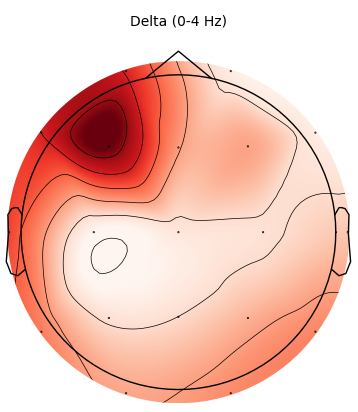
\includegraphics{images/topomap_delta_colored.png}
            \caption{}
        \end{subfigure}
        &
        \begin{subfigure}[c]{0.3\textwidth}
            \centering
            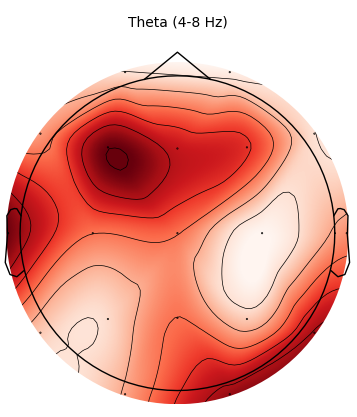
\includegraphics{images/topomap_theta_colored.png}
            \caption{}
        \end{subfigure}
    \end{tabular}
    \vspace{\abovecaptionskip}
    \begin{tabular}{ccc}
        \begin{subfigure}[c]{0.3\textwidth}
            \centering
            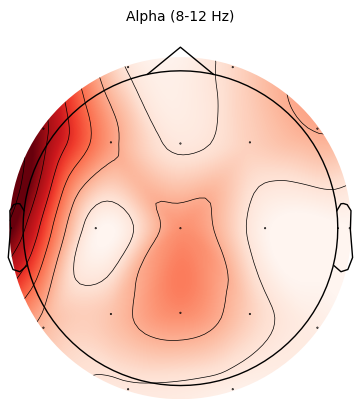
\includegraphics{images/topomap_alpha_colored.png}
            \caption{}
        \end{subfigure}
        &
        \begin{subfigure}[c]{0.3\textwidth}
            \centering
            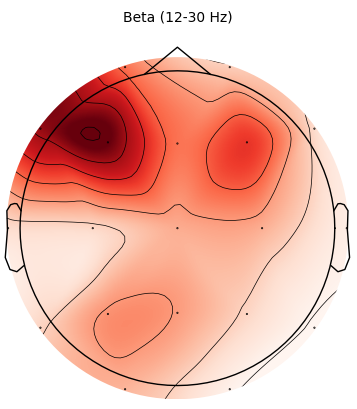
\includegraphics{images/topomap_beta_colored.png}
            \caption{}
        \end{subfigure}
        &
        \begin{subfigure}[c]{0.3\textwidth}
            \centering
            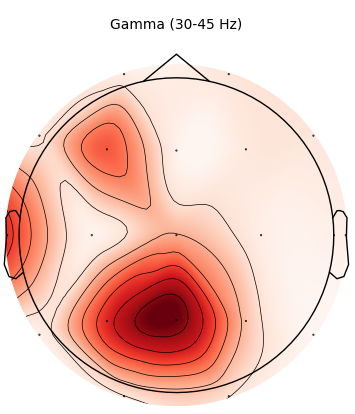
\includegraphics{images/topomap_gamma_colored.png}
            \caption{}
        \end{subfigure}
    \end{tabular}
    \caption{Топографические карты построенные по соответствующим каналам. (а) - Delta-канал (0-4 Гц), (б) - Theta-канал (4-8 Гц), (в) - Alpha-канал (8-12 Гц), (г) - Beta-канал (12-30 Гц), (д) - Gamma-канал (30-45 Гц),}
    \label{fig:topomap_colored}
\end{figure}

Задача предобработки заключается в улучшении качества ЭЭГ-сигналов, для корректного последующего анализа, включая извлечение характеристик, таких как альфа- и бета-ритмы. Недостаточная предобработка может привести к искажению результатов и ошибочным выводам, поэтому этот этап является обязательным в исследовательской практике.

\endinput                                     % Первая глава
\chapter{Анализ данных топографических карт}
\label{ch:chap2}
Программа осуществляет чтение набора временных срезов топографических карт, соответствующих различным каналам ЭЭГ. Затем карты проходят предварительную обработку, включая обрезку и преобразование в черно-белый формат. На следующем этапе выполняется пороговая обработка изображений, что позволяет создать бинарную маску, отображающую активные и неактивные области.

На заключительном этапе временные срезы объединяются в видеоролик, предназначенный для последующего анализа. Также рассчитывается процент площади наименее активных зон для заданного канала, что позволяет оценить пространственно-временные характеристики минимальной активности мозга.
\section{Предобработка}

    \begin{enumerate}
        \item Загрузка данных
        \begin{enumerate}
            \item Чтение всех ранее созданных PNG-файлов в указанной директории
        \end{enumerate}
        \item Графическая обработка PNG-файлов с топографическими картами
        \begin{enumerate}
            \item Преобразование изображений в черно-белый формат по следующей формуле:
                \begin{equation}
                    I_{\text{gray}} = 0.299 \cdot R + 0.587 \cdot G + 0.114 \cdot B,
                    \label{eq:grayscale_conversion}
                \end{equation}
                    
                где:
                \begin{itemize}
                    \item \( I_{\text{gray}} \) — яркость пикселя в градациях серого,
                    \item \( R \) — значение красного канала (Red),
                    \item \( G \) — значение зелёного канала (Green),
                    \item \( B \) — значение синего канала (Blue),
                    \item \( 0.299 \), \( 0.587 \), \( 0.114 \) — веса цветовых каналов, основанные на их вкладe в яркость в соответствии с человеческим восприятием.
                \end{itemize}
            \item Обрезание изображения оптимизации последующей обработки
            \item Применение пороговой фильтрации для изображений по следующей формуле:
                \begin{equation}
                    I_{\text{binary}}(x, y) =
                    \begin{cases} 
                        I_{\text{max}}, & \text{если } I_{\text{input}}(x, y) > T, \\
                        I_{\text{min}}, & \text{иначе,}
                    \end{cases}
                    \label{eq:thresholding}
                \end{equation}

                где:
                \begin{itemize}
                    \item \( I_{\text{binary}}(x, y) \) — значение интенсивности пикселя в двоичном изображении,
                    \item \( I_{\text{input}}(x, y) \) — значение интенсивности пикселя в исходном изображении,
                    \item \( T \) — пороговое значение (\(T = 235\)),
                    \item \( I_{\text{max}} \) — максимальное значение интенсивности (например, \(255\) для 8-битных изображений),
                    \item \( I_{\text{min}} \) — минимальное значение интенсивности (например, \(0\) для 8-битных изображений).
                \end{itemize}
        \end{enumerate}
    \end{enumerate}
    В результате этапа предобработки формируется бинарное изображение топографической карты, на котором зоны с минимальной активностью головного мозга визуализированы в виде выделенных белым цветом областей.
Примеры временных срезов топографических карт для соответствующих каналов: \newline
\begin{figure}[!ht]
    \centering
    \begin{tabular}{cc}
        \begin{subfigure}[c]{0.3\textwidth}
            \centering
            
\includegraphics{images/topomap_delta_binary.png}
            \caption{}
        \end{subfigure}
        &
        \begin{subfigure}[c]{0.3\textwidth}
            \centering
            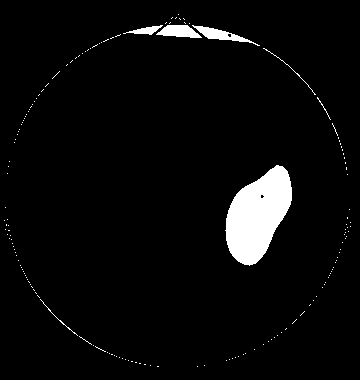
\includegraphics{images/topomap_theta_binary.png}
            \caption{}
        \end{subfigure}
    \end{tabular}
    \vspace{\abovecaptionskip}
    \begin{tabular}{ccc}
        \begin{subfigure}[c]{0.3\textwidth}
            \centering
            
\includegraphics{images/topomap_alpha_binary.png}
            \caption{}
        \end{subfigure}
        &
        \begin{subfigure}[c]{0.3\textwidth}
            \centering
            
\includegraphics{images/topomap_beta_binary.png}
            \caption{}
        \end{subfigure}
        &
        \begin{subfigure}[c]{0.3\textwidth}
            \centering
            
\includegraphics{images/topomap_gamma_binary.png}
            \caption{}
        \end{subfigure}
    \end{tabular}
    \caption{<Бинарные изображения топографических карт из \hyperref[fig:topomap_colored]{Рисунка \ref*{fig:topomap_colored}} построенные по соответствующим каналам. (а) - Delta-канал (0-4 Гц), (б) - Theta-канал (4-8 Гц), (в) - Alpha-канал (8-12 Гц), (г) - Beta-канал (12-30 Гц), (д) - Gamma-канал (30-45 Гц),}
    \label{fig:topomap_binary}
\end{figure}
    
\section{Создание видеоролика}
На данном этапе все сформированные бинарные представления топографических карт последовательно объединяются в видеоролик. Этот процесс позволяет представить динамическое изменение активности головного мозга в удобной визуальной форме, что упрощает анализ временных паттернов и пространственного распределения активности. Использование видеоформата способствует более наглядной интерпретации данных, позволяет отслеживать изменения в различных зонах мозга и улучшает эффективность последующего анализа.

\section{Вычисление неактивной области по временным интервалам}
В рамках обработки данных выполняется расчет доли неактивной области относительно общей площади топографической карты. Этот показатель выражается в процентах и позволяет количественно оценить распределение зон минимальной активности на карте.

Теоретически, неактивные области определяются как регионы с амплитудой сигналов ниже заданного порогового значения, которое устанавливается в зависимости от целей исследования и характеристик данных.

Процесс вычисления основывается на бинарной маске изображения, где активные области представлены единицами, а неактивные — нулями. Соотношение суммарной площади неактивных пикселей к общей площади карты рассчитывается по формуле:

\begin{equation}
P_{\text{inactive}} = \frac{S_{\text{inactive}}}{S_{\text{total}}} \times 100\%,
\end{equation}

где:
\begin{itemize}
    \item \( P_{\text{inactive}} \) — процент неактивной области,
    \item \( S_{\text{inactive}} \) — площадь неактивной области, определяемая как количество пикселей, соответствующих значениям ниже установленного порога,
    \item \( S_{\text{total}} \) — общая площадь топографической карты, выраженная в количестве всех пикселей.
\end{itemize}

Процентное выражение позволяет проводить сравнение между разными временными срезами или картами, что важно для выявления динамических изменений активности мозга.

\endinput                                     % Вторая глава
\chapter{Представление результатов}
\section{Графики процента неактивной области}
    В разделе представления результатов были построены графики, отображающие процент наименее активных зон для различных каналов на каждом временном срезе. Эти графики позволяют визуализировать изменения в пространственно-временной динамике активности мозга.
    \begin{figure}[ht]
        \centering
        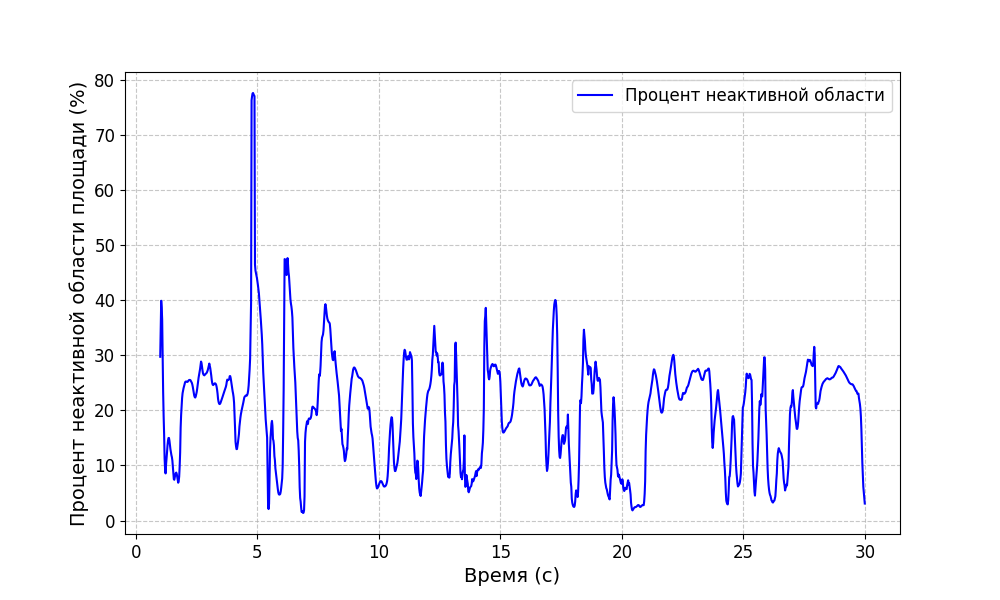
\includegraphics[width=1\textwidth]{images/delta_graphic.png}
        \caption{График, отображающий процент неактивной области для Delta-канала (0-4 Гц)}
        \label{fig:delta_graphic}
    \end{figure}
    \begin{figure}[ht]
        \centering
        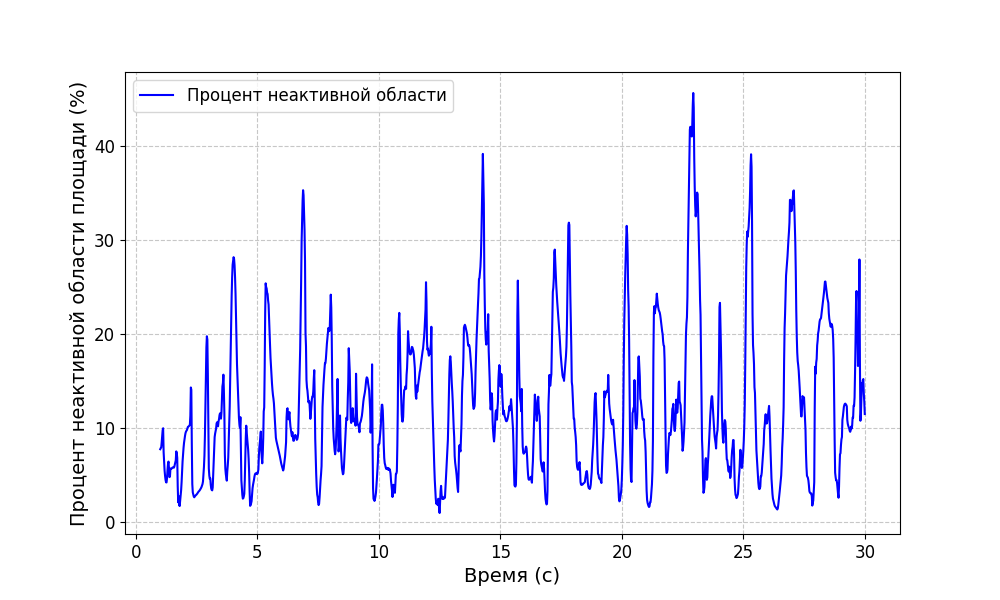
\includegraphics[width=1\textwidth]{images/theta_graphic.png}
        \caption{График, отображающий процент неактивной области для Theta-канала (4-8 Гц)}
        \label{fig:theta_graphic}
    \end{figure}
    \begin{figure}[ht]
        \centering
        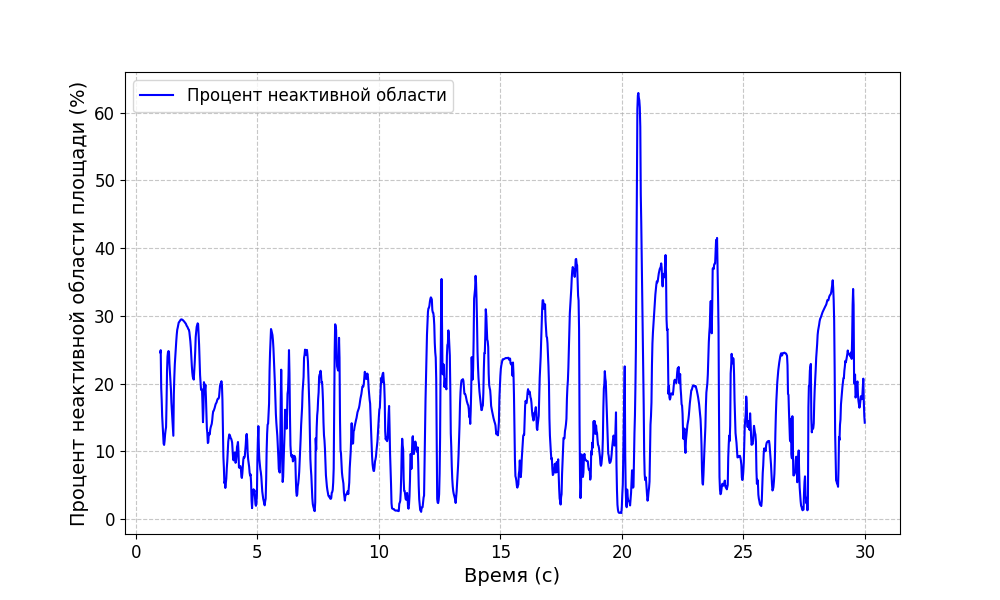
\includegraphics[width=1\textwidth]{images/alpha_graphic.png}
        \caption{График, отображающий процент неактивной области для Alpha-канала (8-12 Гц)}
        \label{fig:alpha_graphic}
    \end{figure}
    \begin{figure}[ht]
        \centering
        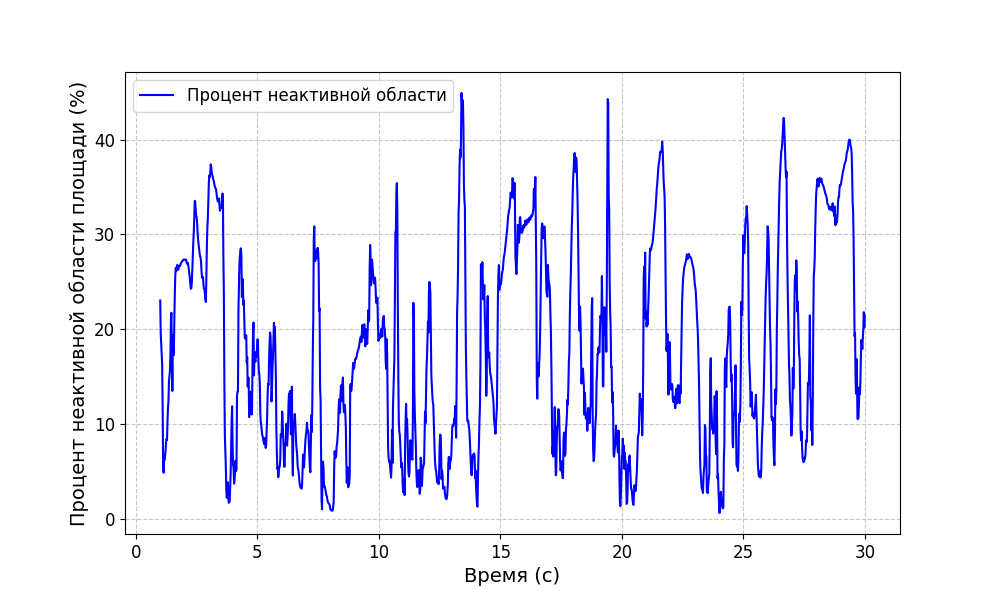
\includegraphics[width=1\textwidth]{images/beta_graphic.png}
        \caption{График, отображающий процент неактивной области для Beta-канала (12-30 Гц)}
        \label{fig:beta_graphic}
    \end{figure}
    \begin{figure}[ht]
        \centering
        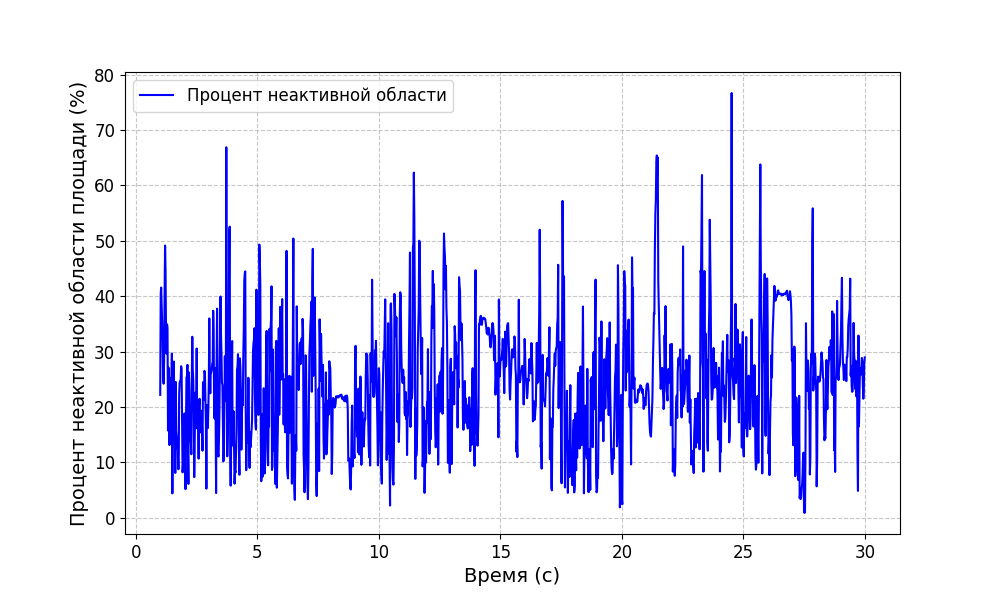
\includegraphics[width=1\textwidth]{images/gamma_graphic.png}
        \caption{График, отображающий процент неактивной области для Gamma-канала (30-45 Гц)}
        \label{fig:gamma_graphic}
    \end{figure}
    
\section{Среднее значение процента неактивной области}
Было вычислено среднее значение процента неактивной области для каждого канала на протяжении всего временного интервала. Полученные данные дают общее представление о характере активности для разных областей мозга, а также помогают выявить закономерности и аномалии в распределении активности в ходе эксперимента.

\begin{table}[ht]
\label{tab:t1}
\centering
\caption{Значение средних показателей процета неактивной области по частотным каналам}
\label{tab:table}
\begin{tabular}{|с|с|}
\hline
Канал    & Среднее значение процента неактивной зоны (\%) \\ \hline
Delta-канал (0-4 Гц)        & 20.11     \\
Theta-канал (4-8 Гц)        & 12.35     \\
Alpha-канал (8-12 Гц)       & 15.97     \\
Beta-канал (12-30 Гц)       & 17.90     \\
Gamma-канал (30-45 Гц)      & 24.01     \\ \hline
\end{tabular}
\end{table}

\section{Видеоролик с изменением топографических карт по времени}
Видео было создано посредством последовательного объединение бинарных изображений топографических карт. Каждое видео создано для отдельных каналов с соответсвующими названиями. Белыми областями представлены неактивные зоны.
\newline
Видео можно посмотреть по следующей \href{https://drive.google.com/drive/folders/1v-PtyjnEAI0c8PzsOospUVqq7BrCfBsq?usp=sharing}{ссылке:}
\newline
https://drive.google.com/drive/folders/1v-PtyjnEAI0c8PzsOospUVqq7BrCfBsq?u
sp=sharing

\endinput                                     % Третья глава
\chapter*{Заключение}
\addcontentsline{toc}{chapter}{Заключение}
\section*{Анализ данных о средних значений процента неактивной области}
По результатам данных из \hyperref[tab:table]{Таблицы 1} можно сделать вывод, что наименее равномерное распределение мощностей сигнала в частотной области определенного канала приходится на delta- и gamma- ритмы. Это отражает нерегулярное расределенеие, что связано с локальными различиями и вовлеченностью отдельных зон мозга для данных ритмов. На примере alpha- и theta- каналов можно наблюдать отсутствие локализированной активности.
\section*{Анализ видеороликов}
Вследствие анализа видеороликов, было выявлено, что наименее активной зоной является центральная зона головного мозга, отвечающая за моторную активность. Это может свидетельствовать о переходе мозга в более спокойное состояние, вследсвие расслабления, или об отсутсвии дивгательной активности.

\endinput                                % Заключение

\begin{thebibliography}{9}
 \bibitem{label1} С. Гонсалес, Р. Вудс "Цифровая обработка изображений". - Москва. - 2012.
\bibitem{label2} Э. Марк, Роберт Ф, "Магнитно-резонансная томография: физические принципы и дизайн последовательности". - Нью-Йорк. - 1999.
\bibitem{mne} MNE-Python documentation: Filtering and preprocessing. \href{https://mne.tools/stable/}{Ссылка}.
\newline
https://mne.tools/stable/

\bibitem{oppenheim} Oppenheim, A. V., Schafer, R. W., \& Buck, J. R. (1999). \textit{Discrete-Time Signal Processing}. Prentice Hall.
\end{thebibliography}
\endinput

\end{document}